% interactapasample.tex
% v1.05 - August 2017
\documentclass[]{interact}

\usepackage{minted} % for HaskellCode
\usepackage{epstopdf}% To incorporate .eps illustrations using PDFLaTeX, etc.
\usepackage[caption=false]{subfig}% Support for small, `sub' figures and tables
%\usepackage[nolists,tablesfirst]{endfloat}% To `separate' figures and tables from text if required
%\usepackage[doublespacing]{setspace}% To produce a `double spaced' document if required
%\setlength\parindent{24pt}% To increase paragraph indentation when line spacing is doubled

% UNCOMMENT WHEN USING BIBITEM
%\usepackage[longnamesfirst,sort]{natbib}% Citation support using natbib.sty
%\bibpunct[, ]{(}{)}{;}{a}{,}{,}% Citation support using natbib.sty
%\renewcommand\bibfont{\fontsize{10}{12}\selectfont}% To set the list of references in 10 point font using natbib.sty
%
% define HaskellCode command for nice formatting of Haskell Code
\newminted[HaskellCode]{haskell}{fontsize=\footnotesize}

\usepackage[natbibapa,nodoi]{apacite}% Citation support using apacite.sty. Commands using natbib.sty MUST be deactivated first!
\setlength\bibhang{12pt}% To set the indentation in the list of references using apacite.sty. Commands using natbib.sty MUST be deactivated first!
\renewcommand\bibliographytypesize{\fontsize{10}{12}\selectfont}% To set the list of references in 10 point font using apacite.sty. Commands using natbib.sty MUST be deactivated first!

\theoremstyle{plain}% Theorem-like structures provided by amsthm.sty
\newtheorem{theorem}{Theorem}[section]
\newtheorem{lemma}[theorem]{Lemma}
\newtheorem{corollary}[theorem]{Corollary}
\newtheorem{proposition}[theorem]{Proposition}

\theoremstyle{definition}
\newtheorem{definition}[theorem]{Definition}
\newtheorem{example}[theorem]{Example}

\theoremstyle{remark}
\newtheorem{remark}{Remark}
\newtheorem{notation}{Notation}

\begin{document}

\articletype{ARTICLE TEMPLATE}% Specify the article type or omit as appropriate

% 1. Author details. All authors of a manuscript should include their full name and affiliation on the cover page of the manuscript. Where available, please also include ORCiDs and social media handles (Facebook, Twitter or LinkedIn). One author will need to be identified as the corresponding author, with their email address normally displayed in the article PDF (depending on the journal) and the online article. Authors’ affiliations are the affiliations where the research was conducted. If any of the named co-authors moves affiliation during the peer-review process, the new affiliation can be given as a footnote. Please note that no changes to affiliation can be made after your paper is accepted. Read more on authorship.
\title{Specification Testing of Agent-Based Simulation using Property-Based Testing.}

\author{
\name{Jonathan Thaler \textsuperscript{a}\thanks{CONTACT Jonathan Thaler. Email: jonathan.thaler@nottingham.ac.uk} and Peer-Olaf Siebers\textsuperscript{a}}
\affil{\textsuperscript{a}School Of Computer Science, University of Nottingham, 7301 Wollaton Rd, Nottingham, UK;}
}

\maketitle

% 2. Should contain an unstructured abstract of 200 words. 
% 3. You can opt to include a video abstract with your article. Find out how these can help your work reach a wider audience, and what to think about when filming.
\begin{abstract}
This paper explores how to use random property-based testing on a technical level to encode and test specifications of agent-based simulations (ABS). The claim is that opposed to unit testing, random property-based testing is a much more natural fit to test ABS due to both stochastic nature. The paper shows how to test full agent- and model-specifications, in the case of an agents behaviour, its transition probabilities and model invariants. The outcome are specifications expressed directly in code, which relate whole classes of random input to expected classes of output. During test execution, random test data is generated automatically, potentially covering the equivalent of thousands of unit tests, run within seconds. The expressiveness and power of property-based testing is not only limited to be part of a test-driven development process where it acts as specification, verification and regression test but can be integrated as a fundamental part of the model development process, supporting the hypothesis and discovery making process. By incorporating this powerful technique into the simulation development process the confidence in the correctness of an implementation increases dramatically, something of fundamental importance for ABS in general and for ABS supporting far-reaching policy decisions in particular.
\end{abstract}

% 4. Between 3 and 6 keywords. Read making your article more discoverable, including information on choosing a title and search engine optimization.
\begin{keywords}
Testing; Test Driven Development; Model Specification;
\end{keywords}

% 5 Funding details - not required for this paper

% 6. Disclosure statement. This is to acknowledge any financial interest or benefit that has arisen from the direct applications of your research. - not required in this paper

% 7. Supplemental online material. Supplemental material can be a video, dataset, fileset, sound file or anything which supports (and is pertinent to) your paper. We publish supplemental material online via Figshare. 
% TODO

% 8. Figures. Figures should be high quality (1200 dpi for line art, 600 dpi for grayscale and 300 dpi for colour, at the correct size). Figures should be supplied in one of our preferred file formats: EPS, PS, JPEG, GIF, or Microsoft Word (DOC or DOCX). For information relating to other file types, please consult our Submission of electronic artwork document.

% 9. Tables. Tables should present new information rather than duplicating what is in the text. Readers should be able to interpret the table without reference to the text. Please supply editable files.

% 10. Equations. If you are submitting your manuscript as a Word document, please ensure that equations are editable. 

% 11. Units. Please use SI units (non-italicized).

% WORD LIMITS: find . -name '*.tex' | xargs wc
% Please include a word count for your paper. A typical article for this journal should be no more than 6000 words; this limit does not include the abstract, endnotes, tables, figures, figure captions and legends, or references. 

\section{Introduction}
There exists a large number of simulation packages which allow the convenient creation of System Dynamics simulations by straight-forward visual diagram creation. One simply creates stocks and flows, connects them, specifies the flow-rates and initial parameters and then runs the model. An example for such a visual diagram creation in the simulation package AnyLogic can be seen in Figure \ref{fig:sir_stockflow_diagram}.

\begin{figure}
	\centering
	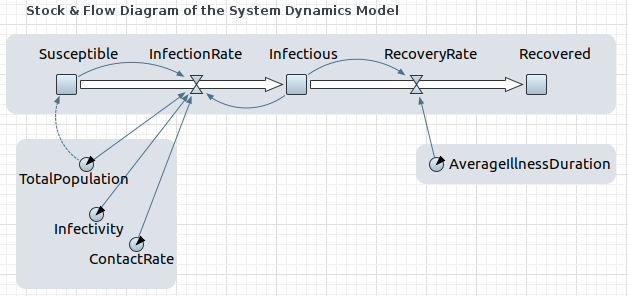
\includegraphics[width=.5\textwidth, angle=0]{./fig/SIR_SD_STOCKFLOW_DIAGRAMM.png}
	\caption{Visual System Dynamics Diagram of the SIR model in AnyLogic Personal Learning Edition 8.3.1.}
	\label{fig:sir_stockflow_diagram}
\end{figure}

Still, implementing System Dynamics directly in code is not as straight forward and involves numerical integration which can be quite tricky to get right. Thus, the aim of this paper is to look into how System Dynamics models can be implemented in code correctly without the use of a simulation package. We use the well known SIR model \cite{kermack_contribution_1927} from epidemiology to demonstrate our approach.

Our language of choice is Haskell because it emphasises a declarative programming style in which one describes \textit{what} instead of \textit{how} to compute. Further it allows to rule out interference with non-deterministic influences or side-effects already at compile-time. This is of fundamental importance for System Dynamics because it behaves completely deterministic and involves no stochastics or non-determinism whatsoever. Also, we make use of Functional Reactive Programming which allows to express continuous-time systems in a functional way. 

We show that by this approach we can arrive at correct-by-construction implementations of System Dynamic models. This means that the correctness of the code is obvious because we have closed the gap between the model specification and its implementation. Thus, the contribution of the paper is the demonstration of how to implement correct-by-construction System Dynamics simulations using Haskell and Functional Reactive Programming.

\section*{Property-Based Testing}
\label{sec:proptesting}

Property-based testing allows to formulate \textit{functional specifications} in code which then a property-based testing library tries to falsify by \textit{automatically} generating test-data, covering as much cases as possible. When a case is found for which the property fails, the library then reduces the test-data to its simplest form for which the test still fails e.g. shrinking a list to a smaller size. It is clear to see that this kind of testing is especially suited to ABS, because we can formulate specifications, meaning we describe \textit{what} to test instead of \textit{how} to test. Also the deductive nature of falsification in property-based testing suits very well the constructive and exploratory nature of ABS. Further, the automatic test-generation can make testing of large scenarios in ABS feasible because it does not require the programmer to specify all test-cases by hand, as is required in e.g. traditional unit tests.

Property-based testing was introduced in \cite{claessen_quickcheck_2000,claessen_testing_2002} where the authors present the QuickCheck library in Haskell, which tries to falsify the specifications by \textit{randomly} sampling the test space. We argue, that the stochastic sampling nature of this approach is particularly well suited to ABS, because it is itself almost always driven by stochastic events and randomness in the agents behaviour, thus this correlation should make it straightforward to map ABS to property-testing.
%The main challenge when using QuickCheck, as will be shown later, is to write \textit{custom} test-data generators for agents and the environment which cover the space sufficiently enough to not miss out on important test-cases.
According to the authors of QuickCheck \textit{"The major limitation is that there is no measurement of test coverage."} \cite{claessen_quickcheck_2000}. Although QuickCheck provides help to report the distribution of test-cases it is not able to measure the coverage of tests in general. This could lead to the case that test-cases which would fail are never tested because of the stochastic nature of QuickCheck. Fortunately, the library provides mechanisms for the developer to measure coverage in specific test-cases where the data and its (expected) distribution is known to the developer. This is a powerful tool for testing randomness in ABS as will be shown in subsequent chapters.

\medskip

As a remedy for the potential coverage problems of QuickCheck, there exists also a deterministic property-testing library called SmallCheck \cite{runciman_smallcheck_2008}, which instead of randomly sampling the test-space, enumerates test-cases exhaustively up to some depth. It is based on two observations, derived from model-checking, that (1) \textit{"If a program fails to meet its specification in some cases, it almost always fails in some simple case"} and (2) \textit{"If a program does not fail in any simple case, it hardly ever fails in any case} \cite{runciman_smallcheck_2008}. This non-stochastic approach to property-based testing might be a complementary addition in some cases where the tests are of non-stochastic nature with a search-space  too large to test manually by unit tests but small enough to enumerate exhaustively. The main difficulty and weakness of using SmallCheck is to reduce the dimensionality of the test-case depth search to prevent combinatorial explosion, which would lead to exponential number of cases. Thus one can see QuickCheck and SmallCheck as complementary instead of in opposition to each other.

\subsection*{A brief overview of QuickCheck}
To give a rough idea on how property-based testing works in Haskell, we give a few examples of property-tests on lists, which are directly expressed as functions in Haskell. Such a function has to return a \textit{Bool} which indicates \textit{True} in case the test succeeds or \textit{False} if not and can take input arguments which data is automatically generated by QuickCheck.

\begin{HaskellCode}
-- concatenation operator (++) is associative
append_associative :: [Int] -> [Int] -> [Int] -> Bool
append_associative xs ys zs = (xs ++ ys) ++ zs == xs ++ (ys ++ zs)

-- the reverse of a reversed list is the original list
reverse_reverse :: [Int] -> Bool
reverse_reverse xs = reverse (reverse xs) == xs

-- reverse is distributive over concatenation (++)
-- this test fails for explanatory reasons, for a correct 
-- property xs and ys need to be swapped on the right-hand side!
reverse_distributive :: [Int] -> [Int] -> Bool
reverse_distributive xs ys = reverse (xs ++ ys) == reverse xs ++ reverse ys

-- running the tests
main :: IO ()
main = do
  quickCheck append_associative
  quickCheck reverse_reverse
  quickCheck reverse_distributive
\end{HaskellCode}

When we run the tests using \textit{main}, we get the following output:

\begin{verbatim}
+++ OK, passed 100 tests.
+++ OK, passed 100 tests.
*** Failed! Falsifiable (after 5 tests and 6 shrinks):    
[0]
[1]
\end{verbatim}

We see that QuickCheck generates 100 test-cases for each property-test and it does this by generating random data for the input arguments. Note that we have not specified any data for our input arguments; QuickCheck is able to provide a suitable data-generator through type-inference: for lists and all the existing Haskell types like Int there exist custom generators already.

QuickCheck generates 100 test-cases by default and requires all to pass - if there is a test-case which fails, the overall property-test fails and QuickCheck shrinks the input to a minimal size for which the case still fails and reports it as a counter example. This is the case in the last property-test \textit{reverse\_distributive} which is wrong as \textit{xs} and \textit{ys} need to be swapped on the right-hand side. In this run, QuickCheck found a counter-example to the property after 5 tests and applied 6 shrinks to find the minimal failing example of \textit{xs = [0]} and \textit{ys = [1]}. If we swap \textit{xs} and \textit{ys}, the property-test passes 100 test-cases just like the other two did. Note that it is possible to configure QuickCheck to generate more or less random test-cases, which can be used to increase the coverage if the sampling space is quite large - this will become useful later.

\subsubsection*{Properties and Generators}
TODO: property
TODO: label
TODO: ==>
TODO: generators

\subsubsection*{Coverage}
TODO: cover with checkCoverage


\section{An event-driven agent-based SIR model}
\label{sec:sirmodel}
The explanatory SIR model is a very well studied and understood compartment model from epidemiology \cite{kermack_contribution_1927}, which allows to simulate the dynamics of an infectious disease like influenza, tuberculosis, chicken pox, rubella and measles spreading through a population. The reason for choosing this model is its simplicity as it is easy to understand fully but complex enough to develop basic concepts of pure functional ABS, which are then extended and deepened in the much more complex Sugarscape model of the next section.

In this model, people in a population of size $N$ can be in either one of the three states \textit{Susceptible}, \textit{Infected} or \textit{Recovered} at a particular time, where it is assumed that initially there is at least one infected person in the population. People interact \textit{on average} with a given rate of $\beta$ other people per time unit and become infected with a given probability $\gamma$ when interacting with an infected person. When infected, a person recovers \textit{on average} after $\delta$ time units and is then immune to further infections. An interaction between infected persons does not lead to reinfection, thus these interactions are ignored in this model. This definition gives rise to three compartments with the transitions seen in Figure \ref{fig:sir_transitions}.

\begin{figure}
	\centering
	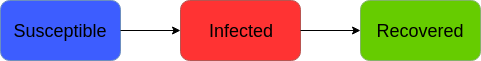
\includegraphics[width=.7\textwidth, angle=0]{./fig/SIR_transitions.png}
	\caption{States and transitions in the SIR compartment model.}
	\label{fig:sir_transitions}
\end{figure}

In this paper we want to implement an agent-based simulation of this model, where we follow TODO: cite macal, translating the informal specification into an an event-driven agent-based approach. 

\begin{figure}
	\centering
	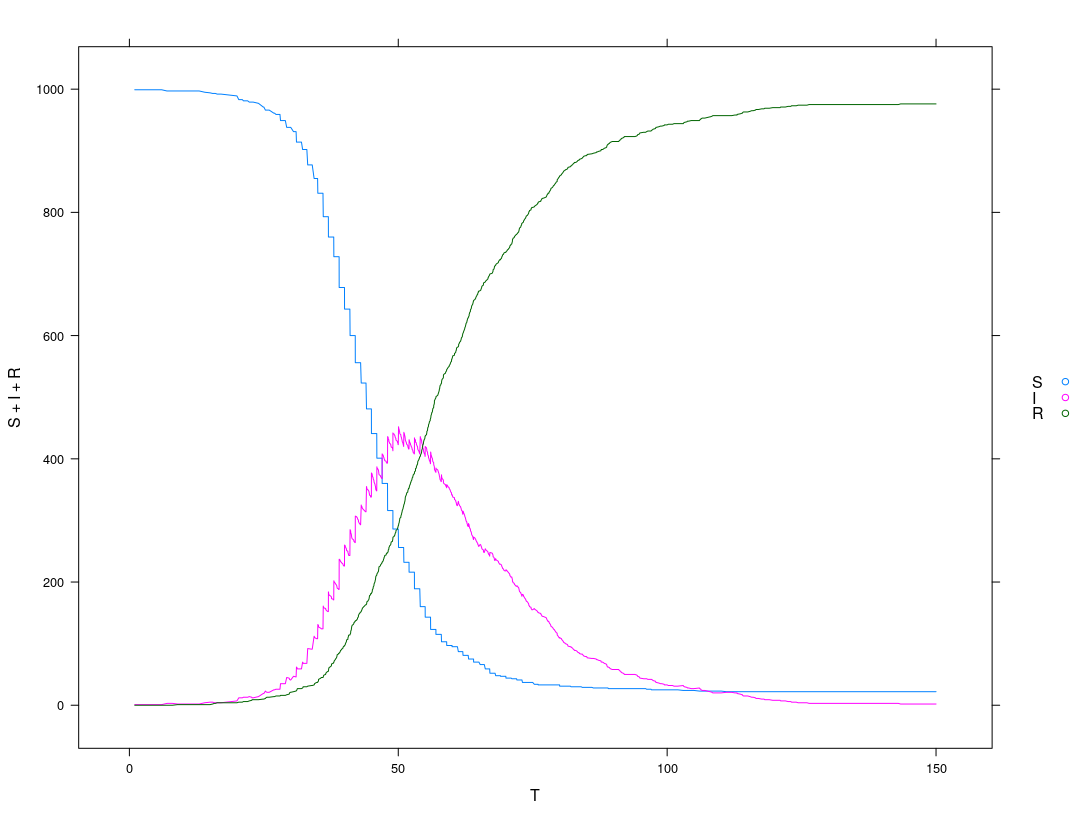
\includegraphics[width=0.7\textwidth, angle=0]{./fig/sir_eventdriven.png}
	\caption{Dynamics of the SIR compartment model using an event-driven agent-based approach. Population Size $N$ = 1,000, contact rate $\beta =  \frac{1}{5}$, infection probability $\gamma = 0.05$, illness duration $\delta = 15$ with initially 1 infected agent.}
	\label{fig:sir_sd_dynamics}
\end{figure}

We start by giving the full \textit{specification} of the susceptible, infected and recovered agent by stating the input-to-output event relations. The susceptible agent is specified as follows:

TODO is there some diagram form (BPNL or other process language, e.g. UML), with which we can express the SIR agents event behaviour? would be more concise than only describing it in word

\begin{enumerate}
	\item \texttt{MakeContact} - if the agent receives this event it will output $\beta$ \texttt{Contact ai Susceptible} events, where \texttt{ai} is the agents own id. The events have to be scheduled immediately without delay, thus having the current time as scheduling timestamp. The receivers of the events are uniformly randomly chosen from the agent population. The agent doesn't change its state, stays \texttt{Susceptible} and does not schedule any other events than the ones mentioned.
	
	\item \texttt{Contact \_ Infected} - if the agent receives this event there is a chance of uniform probability $\gamma$ (infectivity) that the agent becomes \texttt{Infected}. If this happens, the agent will schedule a \texttt{Recover} event to itself into the future, where the time is drawn randomly from the exponential distribution with $\lambda = \delta$ (illness duration). If the agent does not become infected, it will not change its state, stays \texttt{Susceptible} and does not schedule any events.
	
	\item \texttt{Contact \_ \_} or \texttt{Recover} - if the agent receives any of these other events it will not change its state, stays \texttt{Susceptible} and does not schedule any events.
\end{enumerate}

This specification implicitly covers that a susceptible agent can never transition from a \texttt{Susceptible} to a \texttt{Recovered} state within a single event as it can only make the transition to \texttt{Infected} or stay \texttt{Susceptible}. The infected agent is specified as follows:

\begin{enumerate}
	\item \texttt{Recover} - if the agent receives this, it will not schedule any events and make the transition to the \texttt{Recovered} state.
	
	\item \texttt{Contact sender Susceptible} - if the agent receives this, it will reply immediately with \texttt{Contact ai Infected} to \textit{sender}, where \texttt{ai} is the infected agents' id and the scheduling timestamp is the current time. It will not schedule any events and stays \texttt{Infected}.
	
	\item In case of any other event, the agent will not schedule any events and stays \texttt{Infected}.
\end{enumerate}

This specification implicitly covers that an infected agent never goes back to the \texttt{Susceptible} state as it can only make the transition to \texttt{Recovered} or stay \texttt{Infected}. From the specification of the susceptible agent it becomes clear that a susceptible agent who became infected, will always recover as the transition to \texttt{Infected} includes the scheduling of \texttt{Recovered} to itself. 

\medskip

The \textit{recovered} agent specification is very simple. It stays \texttt{Recovered} forever and does not schedule any events.

\section{Encoding Agent Specifications}
\label{sec:method}
We start by encoding the invariants of the susceptible agent directly into Haskell, implementing a function which takes all necessary parameters and returns a \texttt{Bool} indicating whether the invariants hold or not. The encoding is straightforward when using pattern matching and it nearly reads like a formal specification due to the declarative nature of functional programming.

%\begin{HaskellCode}
\begin{footnotesize}
\begin{verbatim}
susceptibleProps :: SIREvent              -- random event sent to agent
                 -> SIRState              -- output state of the agent
                 -> [QueueItem SIREvent]  -- list of events the agent scheduled
                 -> AgentId               -- agent id of the agent
                 -> Bool
-- received Recover => stay Susceptible, no event scheduled
susceptibleProps Recover Susceptible es _ = null es
-- received Contact _ Recovered => stay Susceptible, no event scheduled
susceptibleProps (Contact _ Recovered) Susceptible es _ = null es
-- received Contact _ Susceptible => stay Susceptible, no event scheduled
susceptibleProps (Contact _ Susceptible) Susceptible es _  = null es
-- received Contact _ Infected, didn't get Infected, no event scheduled
susceptibleProps (Contact _ Infected) Susceptible es _ = null es
-- received Contact _ Infected AND got infected, check events
susceptibleProps (Contact _ Infected) Infected es ai
  = checkInfectedInvariants ai es
-- received MakeContact => stay Susceptible, check events
susceptibleProps MakeContact Susceptible es ai
  = checkMakeContactInvariants ai es cor
-- all other cases are invalid and result in a failed test case
susceptibleProps _ _ _ _ = False
\end{verbatim}
\end{footnotesize}
%\end{HaskellCode}

Next, we give the implementation for the \texttt{checkInfectedInvariants} function. We omit a detailed implementation of \texttt{checkMakeContactInvariants} as it works in a similar way and its details do not add anything conceptually new. The function \texttt{checkInfectedInvariants} encodes the invariants which have to hold when the susceptible agent receives a \texttt{(Contact \_ Infected)} event from an infected agent and becomes infected:

%\begin{HaskellCode}
\begin{footnotesize}
\begin{verbatim}
checkInfectedInvariants :: AgentId               -- agent id of the agent 
                        -> [QueueItem SIREvent]  -- list of scheduled events
                        -> Bool
checkInfectedInvariants sender 
  -- expect exactly one Recovery event
  [QueueItem receiver (Event Recover) t'] 
  -- receiver is sender (self) and scheduled into the future
  = sender == receiver && t' >= t 
-- all other cases are invalid
checkInfectedInvariants _ _ = False
\end{verbatim}
\end{footnotesize}
%\end{HaskellCode}

%The \texttt{checkMakeContactInvariants} is a bit more complex:
%
%%%\begin{HaskellCode}
%checkMakeContactInvariants :: AgentId              -- ^ Agent id of the agent 
%                           -> [QueueItem SIREvent] -- ^ Events the agent scheduled
%                           -> Int                  -- ^ Contact Rate
%                           -> Bool
%checkMakeContactInvariants sender es contactRate
%    -- make sure there has to be exactly one MakeContact event and
%    -- exactly contactRate Contact events
%    = invOK && hasMakeCont && numCont == contactRate
%  where
%    (invOK, hasMakeCont, numCont) 
%      = foldr checkMakeContactInvariantsAux (True, False, 0) es
%
%    checkMakeContactInvariantsAux :: QueueItem SIREvent 
%                                  -> (Bool, Bool, Int)
%                                  -> (Bool, Bool, Int)
%    checkMakeContactInvariantsAux 
%        (QueueItem (Contact sender' Susceptible) receiver t') (b, mkb, n)
%      = (b && sender == sender'   -- sender in Contact must be self
%           && receiver `elem` ais -- receiver of Contact must be in agent ids
%           && t == t', mkb, n+1)  -- Contact event is scheduled immediately
%    checkMakeContactInvariantsAux 
%        (QueueItem MakeContact receiver t') (b, mkb, n) 
%      = (b && receiver == sender  -- receiver of MakeContact is agent itself
%           && t' == t + 1         -- MakeContact scheduled 1 timeunit into future
%           &&  not mkb, True, n)  -- there can only be one MakeContact event
%    checkMakeContactInvariantsAux _ (_, _, _) 
%      = (False, False, 0)         -- other patterns are invalid
%%\end{HaskellCode}

\subsection{Writing a Property Test}
After having encoded the invariants into a function, we need to write a QuickCheck property test which calls this function with random test data. Although QuickCheck comes with a lot of data generators for existing types like Strings, Integers, Double, List, it obviously does not have generators for custom types, like the \texttt{SIRState} and \texttt{SIREvent}. Thus, the first step is to write custom data generators, which are suitable for our problem at hand.

There are two ways to do this by either fixing them at compile time writing an \texttt{Arbitrary} instance or writing a run-time generator running in the \texttt{Gen} context. The advantage of having an \texttt{Arbitrary} instance is that the custom data type can then be used as an argument to a function, the advantage of writing a run-time generator is that it can depend on values computed during run time.

First, we write an \texttt{Arbitrary} instance for the \texttt{SIRState}. When writing an \texttt{Arbitrary} instance one needs to provide an implementation for the \texttt{arbitrary} method, which returns a value of the given type for which the instance was implemented for - in our case it is \texttt{SIRState}. This implementation makes use of the \texttt{elements} function, which picks a random element from a non-empty list with uniform probability.

%\begin{HaskellCode}
\begin{footnotesize}
\begin{verbatim}
instance Arbitrary SIRState where
  arbitrary = elements [Susceptible, Infected, Recovered]
\end{verbatim}
\end{footnotesize}
%\end{HaskellCode}

Next we write a custom generator to capture the concept of probabilities. This is necessary because if using a \texttt{Double} as input to a function it would cover the whole range of the type but we want to restrict its random range to $(0,1)$ reflecting a probability. We achieve this by introducing a new type and writing an \texttt{Arbitrary} instance for it. This implementation makes use of the \texttt{choose} function, which returns a random value within the given bounds.

%\begin{HaskellCode}
\begin{footnotesize}
\begin{verbatim}
-- define a new type, representing a probability
newtype Probability = P Double
instance Arbitrary Probability where
  arbitrary = P <$> choose (0, 1)
\end{verbatim}
\end{footnotesize}
%\end{HaskellCode}
%$

What is left is to write a custom generator for generating random events. In this case we want to be able to control the distribution of events generated. Instead of using \texttt{elements}, which picks uniformly, if a skewed distribution is needed, one can use the \texttt{frequency} function, where a frequency can be specified for each element. Due to the fact, that event generation is parametrised by frequencies and requires the population ids to pick from in the \texttt{Contact} event, it needs to be a run-time generator, thus running in \texttt{Gen} context. The function takes the frequencies for all three types of events, the frequencies of the \texttt{SIRState} in the \texttt{Contact} event and the agent population to pick the sender id from in the \texttt{Contact} event.

TODO: this is by far too much detail, simply use a uniformly distributed Event generator, as we are only using uniformly distributed events throughout this paper

%\begin{HaskellCode}
\begin{footnotesize}
\begin{verbatim}
genEventFreq :: Int             -- MakeContact frequency
             -> Int             -- Contact frequency
             -> Int             -- Recover frequency
             -> (Int, Int, Int) -- Susceptible, Infected, Recovered frequency
             -> [AgentId]       -- population agent ids
             -> Gen SIREvent
genEventFreq mf cf rf (s,i,r) ais
  -- generate one of the three events with given frequency
  = frequency [ (mf, return MakeContact)
              , (cf, do
                  -- pick SIRState for Contact event
                  ss <- frequency [ (s, return Susceptible)
                                  , (i, return Infected)
                                  , (r, return Recovered)]
                  -- pick sender id for Contact event
                  ai <- elements ais
                  return (Contact ai ss))
              , (rf, return Recover)]
         
-- helper function with uniform frequencies for all events and SIRState
genEvent :: [AgentId] -> Gen SIREvent
genEvent = genEventFreq 1 1 1 (1,1,1) 
\end{verbatim}
\end{footnotesize}
%\end{HaskellCode}

We are now equipped with all functionality to implement the property test. All parameters to the property test are generated randomly, which expresses that the properties encoded in the previous section have to hold invariant of the model parameters. We make use of additional data generator modifiers: \texttt{Positive} ensures that a value generated is positive; \texttt{NonEmptyList} ensures that a randomly generated list is not empty. Further, we use the function \texttt{label}, which can be used to generate labels for a test case, counting occurrences of same labels, generating a histogram. This is useful to get an insight into the distribution of the property test data and we use it to get an understanding for the distribution of the transitions. The case where the agents output state is \texttt{Recovered} is marked as "INVALID" as it must never occur, otherwise the test will fail, due to the invariants encoded in the previous section.

%\begin{HaskellCode}
\begin{footnotesize}
\begin{verbatim}
prop_susceptible :: Positive Int         -- beta (contact rate)
                 -> Probability          -- gamma (infectivity)
                 -> Positive Double      -- delta (illness duration)
                 -> Positive Double      -- current simulation time
                 -> NonEmptyList AgentId -- population agent ids
                 -> Gen Bool
prop_susceptible 
  (Positive beta) (P gamma) (Positive delta) (Positive t) (NonEmpty ais) = do
  -- generate random event, requires the population agent ids
  evt <- genEvent ais
  -- run susceptible random agent with given parameters (implementation omitted)
  (ai, ao, es) <- genRunSusceptibleAgent beta gamma delta t ais evt
  -- check properties
  return (label (labelTestCase ao) (susceptibleProps evt ao es ai))
  where
    labelTestCase :: SIRState -> String
    labelTestCase Infected    = "Susceptible -> Infected"
    labelTestCase Susceptible = "Susceptible"
    labelTestCase Recovered   = "INVALID"
\end{verbatim}
\end{footnotesize}
%\end{HaskellCode}

We have omitted the implementation of \texttt{genRunSusceptibleAgent} as it would require the discussion of implementation details of the agent. Conceptually speaking, it executes the agent with the respective arguments with a fresh random-number generator and returns the agent id, its state and scheduled events it has output.

Finally we can run the test using QuickCheck. Due to the large random sampling space with 5 parameters, we increase the number of test cases to generate to 100,000.

\begin{footnotesize}
\begin{verbatim}
> quickCheckWith (stdArgs {maxSuccess=100000}) prop_susceptible
+++ OK, passed 100000 tests (6.77s):
94.522% Susceptible
 5.478% Susceptible -> Infected
\end{verbatim}
\end{footnotesize}

All 100,000 test cases pass, taking 6.7 seconds to run on our hardware. The distribution of the transitions shows that we indeed cover both cases a susceptible agent can exhibit within one event. It either stays susceptible or makes the transition to infection. The fact that there is no transition to recovered shows that the implementation is correct - for a transition to recovered we would need to send an additional, second event to the agent.

Encoding of the invariants and writing property tests for the infected agents follows the same idea and is not repeated here. Next, we show how to test transition probabilities using the powerful statistical hypothesis testing feature of QuickCheck.

\subsection{Encoding Transition Probabilities}
In the specifications from the previous section there are probabilistic state transitions, for example the susceptible agent \textit{might} become infected, depending on the events it receives and the infectivity ($\gamma$) parameter. We look now into how we can encode these probabilistic properties using the powerful \texttt{cover} feature of QuickCheck.

The function \texttt{cover :: Double $\rightarrow$ Bool $\rightarrow$ String $\rightarrow$ prop $\rightarrow$ Property} allows to explicitly specify that a given percentage of successful test cases belong to a given class. The first argument is the expected percentage; the second argument indicates whether the current test case belongs to the class or not; the third argument is a label for the coverage; the fourth argument is the property which needs to hold for the test case to succeed.

An example would be to use it to check whether at least 15\% of all test cases of the \texttt{prop\_reverse\_reverse} property of section \ref{sec:proptesting} has a length of at least 50. This would be encoded in the following way:

% stack ghci --package QuickCheck
%\begin{HaskellCode}
\begin{footnotesize}
\begin{verbatim}
prop_reverse_reverse_cover :: [Int] -> Property
prop_reverse_reverse_cover xs  =  
  cover 15 (length xs >= 50) "length at least 50" (reverse (reverse xs) == xs)
\end{verbatim}
\end{footnotesize}
%\end{HaskellCode}

%When running it, the output indicates that although all tests passes, as the property is satisfied in all 100 test cases but the expected coverage differs from the actual one.
%
%\begin{footnotesize}
%\begin{verbatim}
%> quickCheck prop_reverse_reverse_cover
%+++ OK, passed 100 tests (0.01s)
%Only 9% length of list at least 50, but expected 15%
%\end{verbatim}
%\end{footnotesize}

For our case we follow a slightly different approach: we include all test cases into the expected coverage, setting the second parameter always to \texttt{True} and we also set the last argument to \texttt{True} as we are only interested in testing the coverage, which is in fact the property we want to test. Implementing this property test is then simply a matter of computing the probabilities and of case analysis over the random input event and the agents output. It is important to note that in this property test we cannot randomise the model parameters $\beta$, $\gamma$ and $\delta$ because this would lead to random coverage. This might seem like a disadvantage but we do not really have a choice here, still the fixed model parameters can be adjusted arbitrarily and the property must still hold. We could have combined this test into the previous one but then we couldn't have used randomised model parameters. For this reason, and to keep the concerns separated we opted for two different tests, which makes them also much more readable. 

%\begin{HaskellCode}
\begin{footnotesize}
\begin{verbatim}
prop_susceptible_prob :: Positive Double       -- current simulation time
                      -> NonEmptyList AgentId  -- population agent ids 
                      -> Property
prop_susceptible_prob (Positive t) (NonEmpty ais) = do
  -- fixed model parameters, otherwise random coverage
  let cor = 5     -- contact rate (beta)
      inf = 0.05  -- infectivity (gamma)
      ild = 15.0  -- illness duration (delta)
  -- compute distributions for all cases depending on event and SIRState
  -- frequencies; technical detail, omitted for clarity reasons
  let recoverPerc       = ...
      makeContPerc      = ...
      contactRecPerc    = ...
      contactSusPerc    = ...
      contactInfSusPerc = ...
      contactInfInfPerc = ...
  -- generate a random event
  evt <- genEvent ais
  -- run susceptible random agent with given parameters, only
  -- interested in its output SIRState, ignore id and events
  (_, ao, _) <- genRunSusceptibleAgent cor inf ild t ais evt
  -- encode expected distributions
  return $ property $ case evt of 
    Recover -> 
      cover recoverPerc True "Susceptible recv Recover" True
    MakeContact -> 
      cover makeContPerc True "Susceptible recv MakeContact" True
    (Contact _ Recovered) -> 
      cover contactRecPerc True "Susceptible recv Contact * Recovered" True
    (Contact _ Susceptible) -> 
      cover contactSusPerc True "Susceptible recv Contact * Susceptible" True
    (Contact _ Infected) -> 
      case ao of
        Susceptible ->
          cover contactInfSusPerc True 
            "Susceptible recv Contact * Infected, stays Susceptible" True
        Infected ->
          cover contactInfInfPerc True 
            "Susceptible recv Contact * Infected, becomes Infected" True
        _ ->
          cover 0 True "INVALID" True
\end{verbatim}
\end{footnotesize}
%\end{HaskellCode}

We have omitted the details of computing the respective distributions of the cases, which depend on the frequencies of the events and the occurrences of \texttt{SIRState} within the \texttt{Contact} event. By varying different distributions in the \texttt{genEvent} function, we can change the distribution of the test cases, leading to a more general test than just using uniform distributed events. When running the property test we get the following output:

\begin{footnotesize}
\begin{verbatim}
+++ OK, passed 100 tests (0.01s):
40% Susceptible recv MakeContact
25% Susceptible recv Recover
14% Susceptible recv Contact * Infected, stays Susceptible
12% Susceptible recv Contact * Susceptible
 9% Susceptible recv Contact * Recovered
    
Only 9% Susceptible recv Contact * Recovered, but expected 11%
Only 25% Susceptible recv Recover, but expected 33%
\end{verbatim}
\end{footnotesize}

QuickCheck runs 100 test cases, prints the distribution of our labels and issues warnings in the last two lines that generated and expected coverages differ in these cases. Further, not all cases are covered, for example the contact with an infected and becoming infected. The reason for these issues is insufficient testing coverage as 100 test cases are simply not enough for a statistically robust result. We could increase the number of test cases to run to 100,000 which will cover then all cases but still QuickCheck is not satisfied as the expected and generated coverage differs in some fractions. % The usage pattern of \texttt{cover}, where we unconditionally include the test case into the coverage class so all test cases pass, emulates failure. 

\medskip

As a solution to this fundamental problem, QuickCheck provides the function \texttt{checkCoverage :: prop $\rightarrow$ Property}. When our property is checked together with \texttt{checkCoverage}, QuickCheck will run as many test cases necessary until it is clear whether the percentage in \texttt{cover} was reached or cannot be reached at all. This is implemented in QuickCheck through sequential statistical hypothesis testing \cite{wald_sequential_1992}. Thus, if QuickCheck comes to the conclusion that the given percentage can or cannot be reached, it is based on a robust statistical test giving strong confidence in the result. With the usage of \texttt{checkCoverage} we get the following output:

\begin{footnotesize}
\begin{verbatim}
+++ OK, passed 819200 tests (7.32s):
33.3292% Susceptible recv Recover
33.2697% Susceptible recv MakeContact
11.1921% Susceptible recv Contact * Susceptible
11.1213% Susceptible recv Contact * Recovered
10.5356% Susceptible recv Contact * Infected, stays Susceptible
 0.5520% Susceptible recv Contact * Infected, becomes Infected
\end{verbatim}
\end{footnotesize}

After 819,200 (!) test cases, run in 7.32 seconds on our hardware, QuickCheck comes to the statistically robust conclusion that the distributions generated by the test cases reflect the expected distributions and passes the property test.

\section{Encoding Model Invariants}
\label{sec:enc_model_inv}
By informally reasoning about the agent specification and by realising that they are, in fact, a state machine with a one-directional flow of \textit{Susceptible} $\rightarrow$ \textit{Infected} $\rightarrow$ \textit{Recovered}, we can come up with a few invariants which have to hold for any SIR simulation run, \textit{under random model parameters} and independent of the random-number stream and the population:

\begin{enumerate}
	\item Simulation time is monotonic increasing. Each event carries a timestamp when it is scheduled. This timestamp may stay constant between multiple events but will eventually increase and must never decrease. Obviously, this invariant is a fundamental assumption in most simulations where time advances into the future and does not flow backwards.
	
	\item The number of total agents $N$ stays constant. In the SIR model no dynamic creation or removal of agents during simulation happens. This is in contrast to the Sugarscape where, depending on the model parameters, this can be very well the case.
	
	\item The number of susceptible agents $S$ is monotonic decreasing. Susceptible agents \textit{might} become infected, reducing the total number of susceptible agents but they can never increase because neither an infected nor recovered agent can go back to susceptible.
	
	\item The number of recovered agents $R$ is monotonic increasing. This is because infected agents \textit{will} recover, leading to an increase of recovered agents but once the recovered state is reached, there is no escape from it.
	
	\item The number of infected agents $I$ respects the invariant of the equation $I = N - (S + R)$ for every step. This follows directly from the first property which says $N = S + I + R$.
\end{enumerate}

\subsection{Encoding the Invariants}
All of those properties are easily expressed directly in code and read like a formal specification due to the declarative nature of functional programming:

%\begin{HaskellCode}
\begin{footnotesize}
\begin{verbatim}
sirInvariants :: Int                    -- N total number of agents
              -> [(Time,(Int,Int,Int))] -- output each step: (Time,(S,I,R))
              -> Bool
sirInvariants n aos = timeInc && aConst && susDec && recInc && infInv
  where
    (ts, sirs)  = unzip aos
    (ss, _, rs) = unzip3 sirs

    -- 1. time is monotonic increasing
    timeInc = allPairs (<=) ts
    -- 2. number of agents N stays constant in each step
    aConst = all agentCountInv sirs
    -- 3. number of susceptible S is monotonic decreasing
    susDec = allPairs (>=) ss
    -- 4. number of recovered R is monotonic increasing
    recInc = allPairs (<=) rs
    -- 5. number of infected I = N - (S + R)
    infInv = all infectedInv sirs

    agentCountInv :: (Int,Int,Int) -> Bool
    agentCountInv (s,i,r) = s + i + r == n

    infectedInv :: (Int,Int,Int) -> Bool
    infectedInv (s,i,r) = i == n - (s + r)

    allPairs :: (Ord a, Num a) => (a -> a -> Bool) -> [a] -> Bool
    allPairs f xs = all (uncurry f) (pairs xs)

    pairs :: [a] -> [(a,a)]
    pairs xs = zip xs (tail xs)
\end{verbatim}
\end{footnotesize}
%\end{HaskellCode}

Putting this property into a QuickCheck test is straightforward. We randomise the model parameters $\beta$ (contact rate), $\gamma$ (infectivity) and $\delta$ (illness duration) because the properties have to hold for all positive, finite model parameters.

%\begin{HaskellCode}
\begin{footnotesize}
\begin{verbatim}
prop_sir_invariants :: Positive Int    -- beta, contact rate
                    -> Probability     -- gamma, infectivity in range (0,1)
                    -> Positive Double -- delta, illness duration
                    -> TimeRange       -- random duration in range (0, 50)
                    -> [SIRState]      -- population
                    -> Property
prop_sir_invariants 
    (Positive beta) (P gamma) (Positive delta) (T t) as  = property (do
  -- total agent count
  let n = length as
  -- run the SIR simulation with a new RNG 
  ret <- genSimulationSIR as beta gamma delta t
  -- check invariants and return result
  return (sirInvariants n ret)
\end{verbatim}
\end{footnotesize}
%\end{HaskellCode}

Due to the large sampling space, we increase the number of test cases to run to 100,000 and all tests pass as expected. It is important to note that we put a random time limit within the range of (0,50) on the simulations to run. Meaning, that if a simulation does not terminate before that limit, it will be terminated at that random \texttt{t}. The reason for this is entirely practical as it ensures that the wall clock time to run the tests stays within reasonable bounds while still retaining randomness. In fact, limiting the duration is actually not necessary because we can reason that the SIR simulation \textit{will always} reach an equilibrium in finite steps. TODO: more argument on this detail

\section{Discussion}
Although there are similarities to the work of \cite{botta_time_2010} (the use of messages and the problem of when to advance time in models with arbitrary number synchronised agent-interactions), we approach our agents differently. First in our approach an agent is only a single MSF and thus can not be directly queried for its internal state / its id or outgoing messages, instead of taking a list of messages, our agents take a single event/message and can produce an arbitrary number of outgoing messages together with an observable state - note that this would allow to query the agent for its id and its state as well by simply sending a corresponding message to the agents MSF and requiring the agent to implement message handling for it. Also the state of our agents is \textit{completely} localised and there is no means of accessing the state from outside the agent, they are thus "fully encapsulated agents" \cite{botta_time_2010}. Note that the authors of \cite{botta_time_2010} define their agents with a polymorphic agent-state type \textit{s}, which implies that without knowledge of the specific type of \textit{s} there would be no way of accessing the state, rendering it in fact also fully encapsulated. The problem of advancing time in our approach is solved not exactly the same but conceptually it is the same: after sending a tick message to each agent (in random order), we process all agents until they are idle: there are no more enqueued messages / events in the queue.

our eventdriven approach makes heavy use of 2 state monads, thus one might ask what the benefits are, after all we seem to fall back into stateful, imperative style programming. we agree that our approach is just one way of implementing abs in fp but we think we have come a long way thus making our approach quite valuable even if there might be other approaches like shallow EDSLs. on the other hand even our stateful programming is highly restricted to only those 2 local datatypes which makes it much more manageable than unrestricted data mutation

quote carmack (\url{http://www.gamasutra.com/view/news/169296/Indepth_Functional_programming_in_C.php}): the main difficulty as a developer in software programming is to keep track of the states a program can be in and reason about them and their Validity

TODO: report LoC and compare it with other implementations we found on the internet

\chapter{Conclusions}
\label{chap:concl}

\section{Being Realistic}
It is of most importance to stress that we don't condemn the current state-of-the-art approach of object-oriented specification and implementation to ABS. The strength of object-oriented programming is surely that it can be seen as \textit{programming as modelling} and thus will be always an attractive approach to ABS. Also we are realists and know that there are more points to consider when selecting a set of methods for developing software for an ABS than robustness, verification and validation. Almost always the popularity of an existing language and which languages the implementer knows is the driving force behind which methods and languages to choose. This means that ABS will continue to be implemented in object-oriented programming languages and many perfectly well functioning models will be created by it in the future. Although they all suffer from the same issues mentioned in the introduction this doesn't matter as they are not of central importance to most of them.
Nonetheless we think our work is still essential and necessary as it may start a slow paradigm-shift and opens up the minds of the ABS community to a more functional and formal way of approaching and implementing agent-based models and simulations and recognizing the benefits one gets automatically from it by doing so.

\section{What we are not doing}
Because of this highly interdisciplinary topic we explicitly mention what we do not want to undertake in this PhD.
First we don't want to develop another language for formal agent-specification which needs to be compiled or used in some fancy tool - we want to put it directly into Haskell, building on the existing facilities.
Second, we are not developing a new economic theory about decentralized bilateral bartering, we take the existing theory and existing agent-based models and apply our methods to them.
Third, we don't want to use fancy statistics and number juggling for comparing validating and verifying models: we want structural comparison (category-theory).
Fourth, we do NOT want to do a direct comparison of object-orientation vs. functional in ABS, as we would get lost in an infinite amount of low-level technical details. We look at the benefits / drawbacks more on a conceptual level, applied to ABS.

\bibliographystyle{apacite}
\bibliography{references}

\end{document}